\section{レポート課題3}
\subsection{課題1}
ロジスティク写像の初期変動の影響がないリターンマップを描くためのプログラムを作成し、個体数変動のリターンマップを表示せよ。このとき $r$ は、$r = 1.50, r = 2.60, r = 3.20, r = 3.50, r = 3.86, r = 3.90$ のとし、初期値$x_0$はランダムに与えなさい。グラフは、授業資料を参考として、 $x_{n+1} = r(1 − x_n)x_n、x_{n+1} = x_n$ も同時に描画し、縦軸と横軸は $0~1$ の範囲で出力すること。\\
画像:\\
\begin{figure}[htbp]
  \begin{tabular}{cc}
    \begin{minipage}[t]{0.45\hsize}
      \centering
      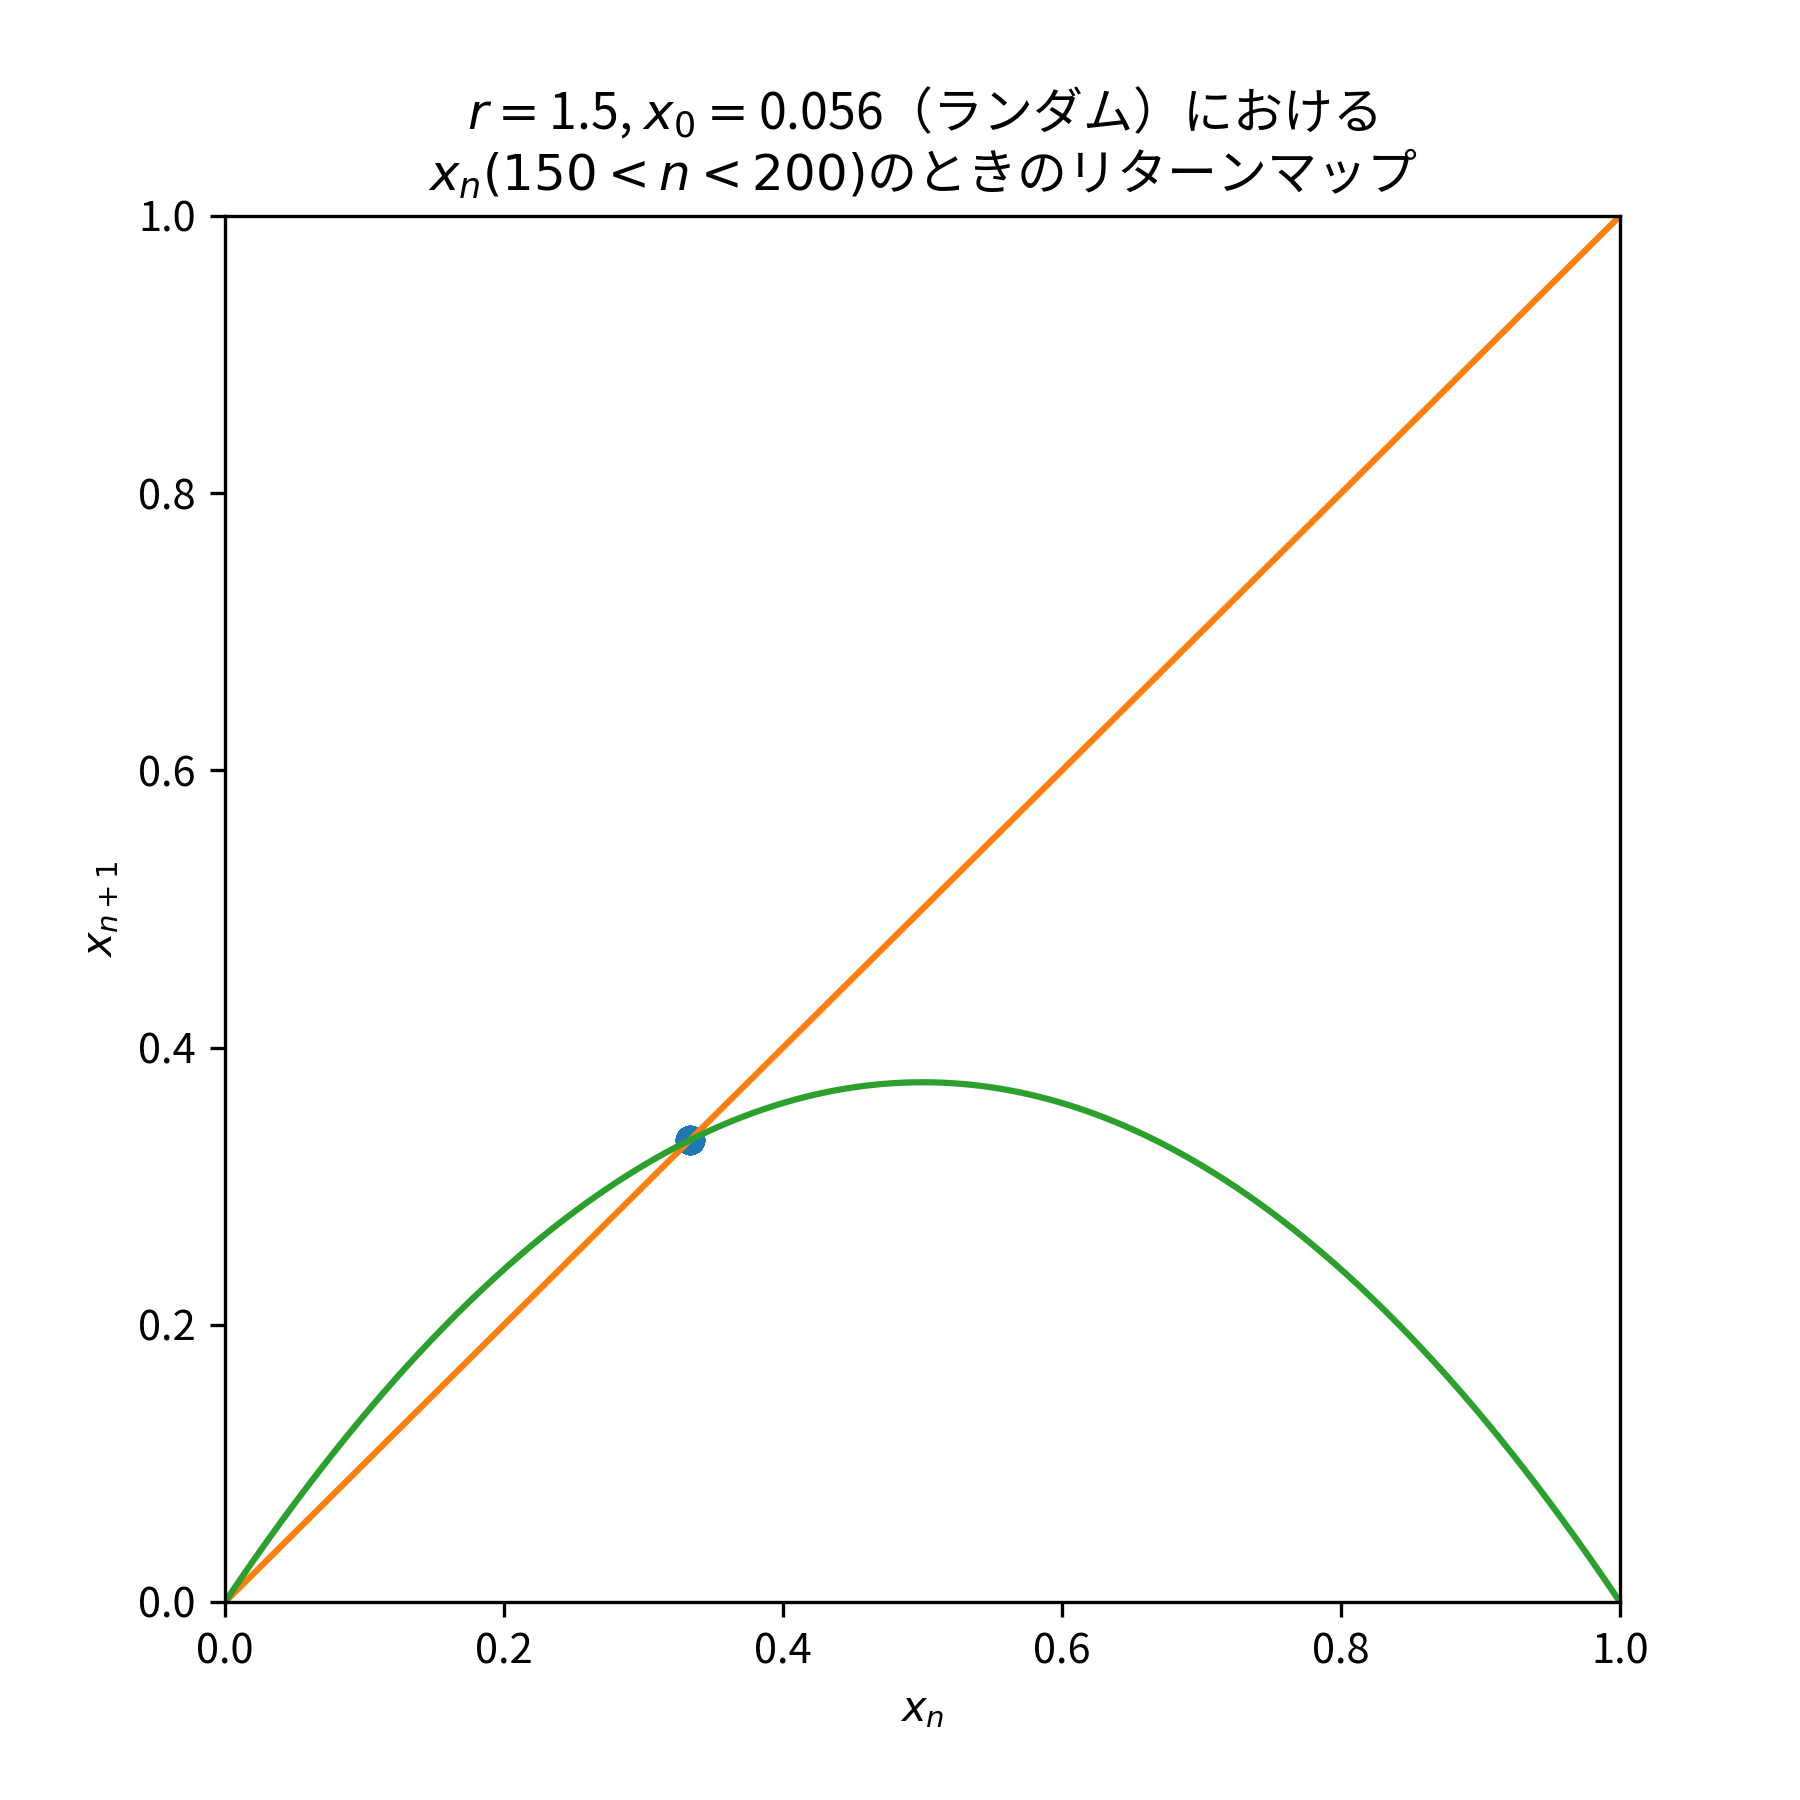
\includegraphics[keepaspectratio, scale=0.3]{images/Problem3/report4_1.png}
    \end{minipage} &
    \begin{minipage}[t]{0.45\hsize}
      \centering
      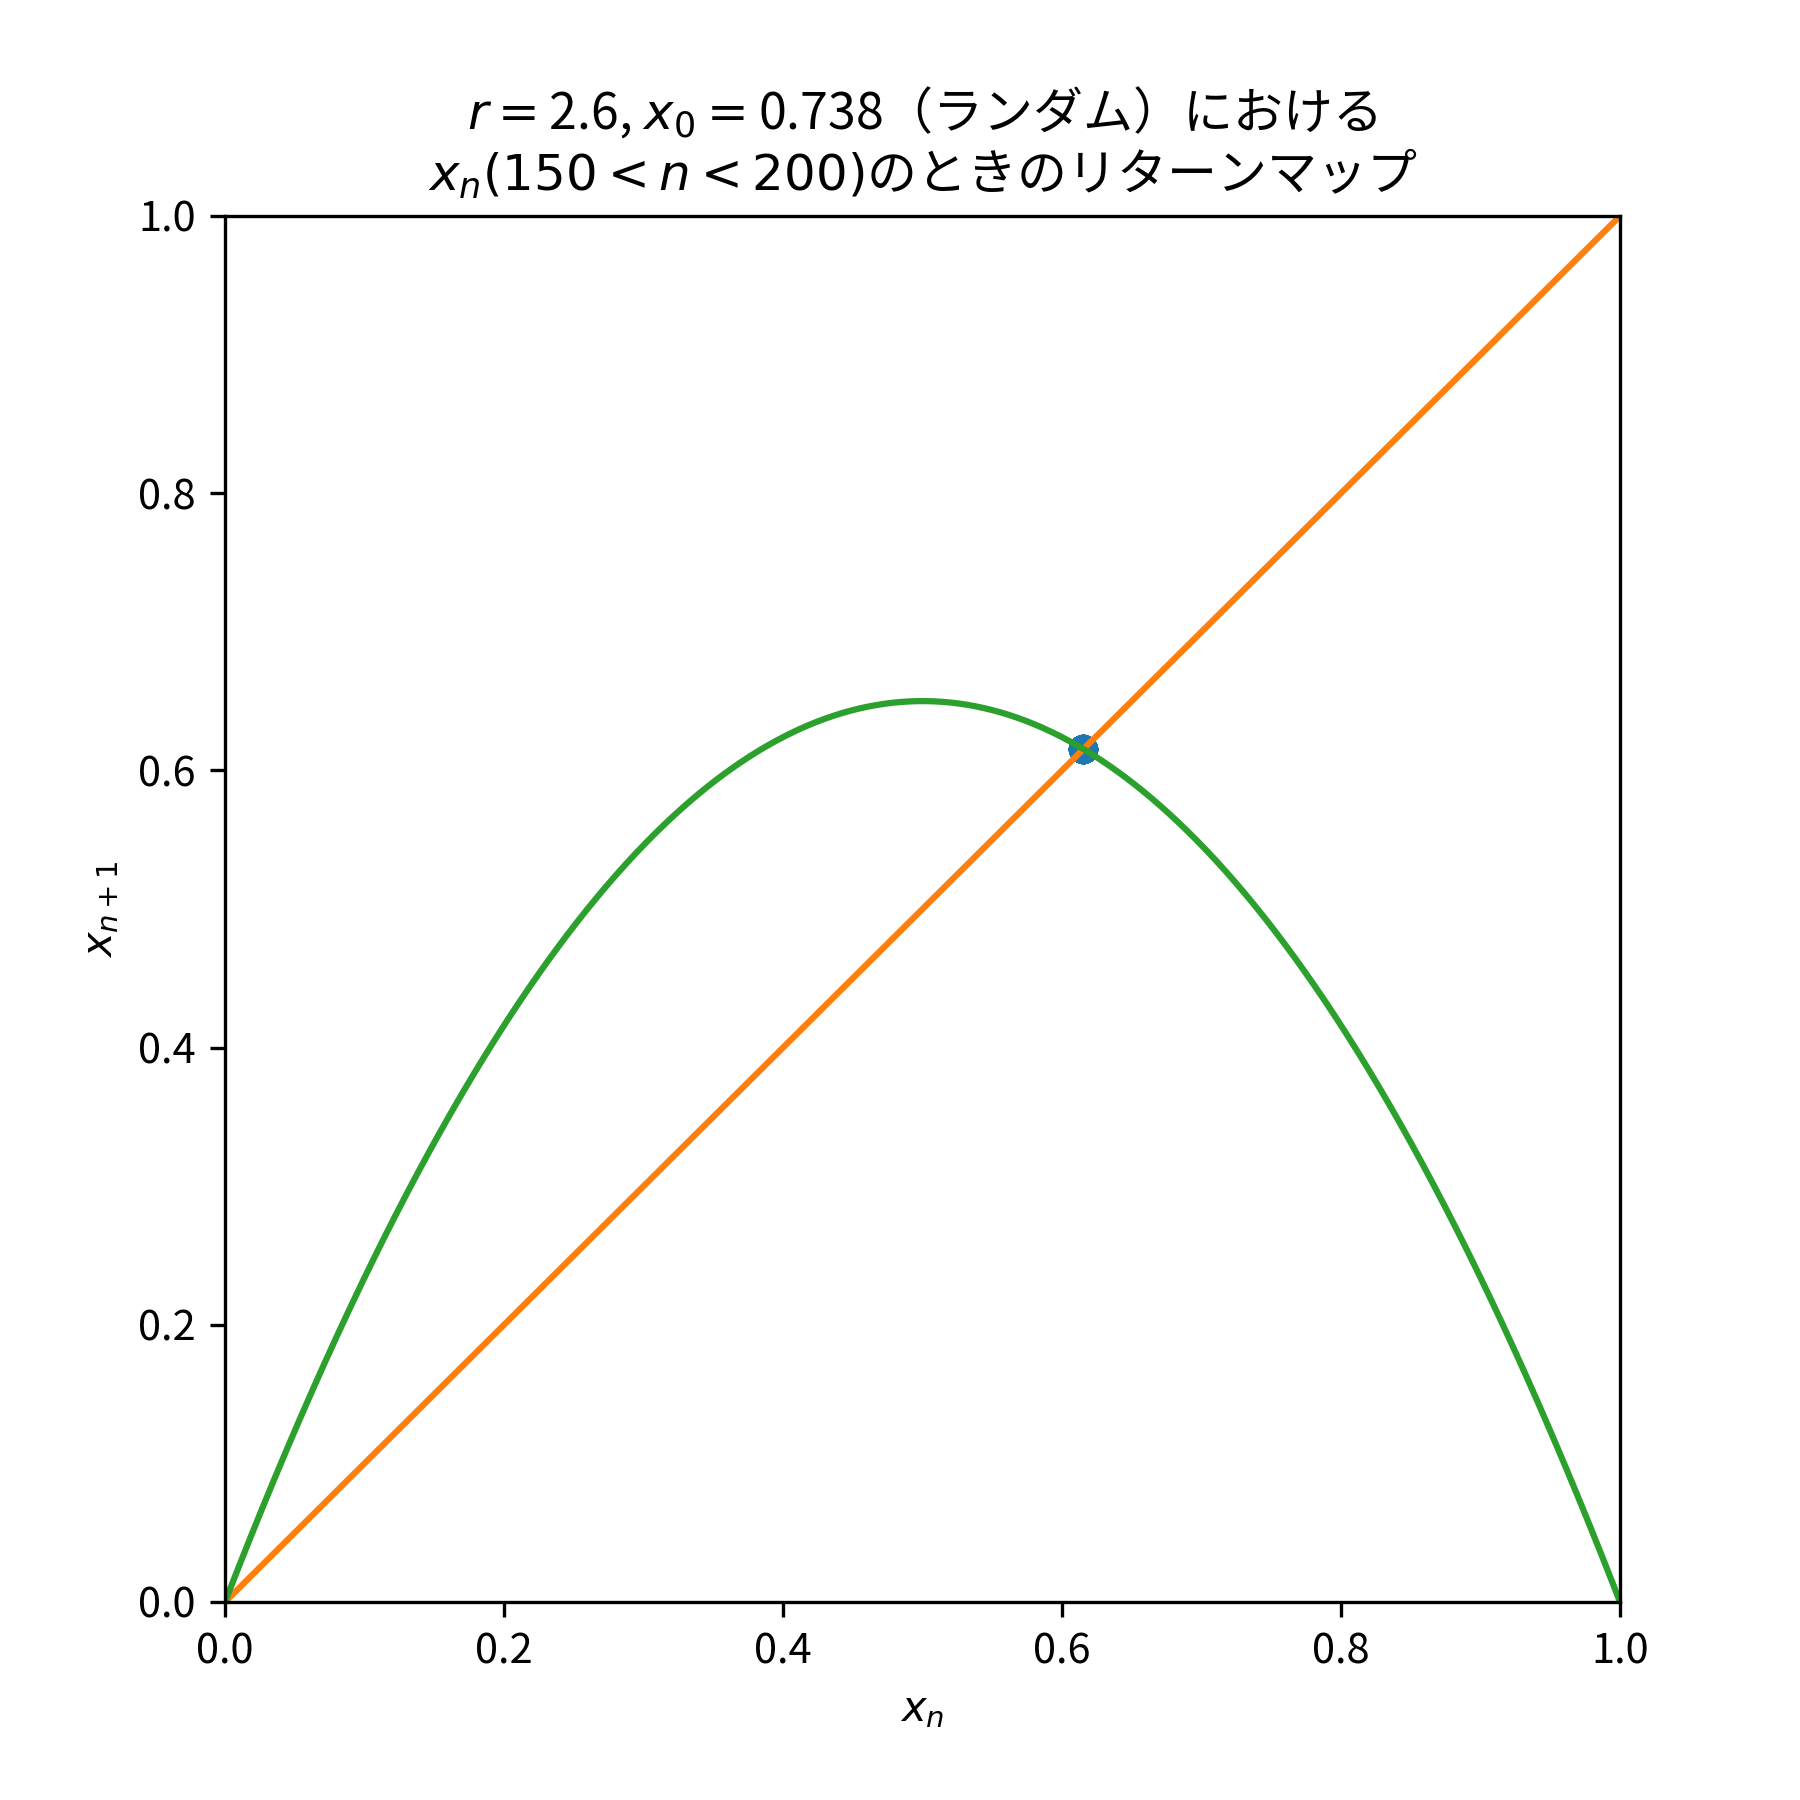
\includegraphics[keepaspectratio, scale=0.3]{images/Problem3/report4_2.png}
    \end{minipage} \\

    \begin{minipage}[t]{0.45\hsize}
      \centering
      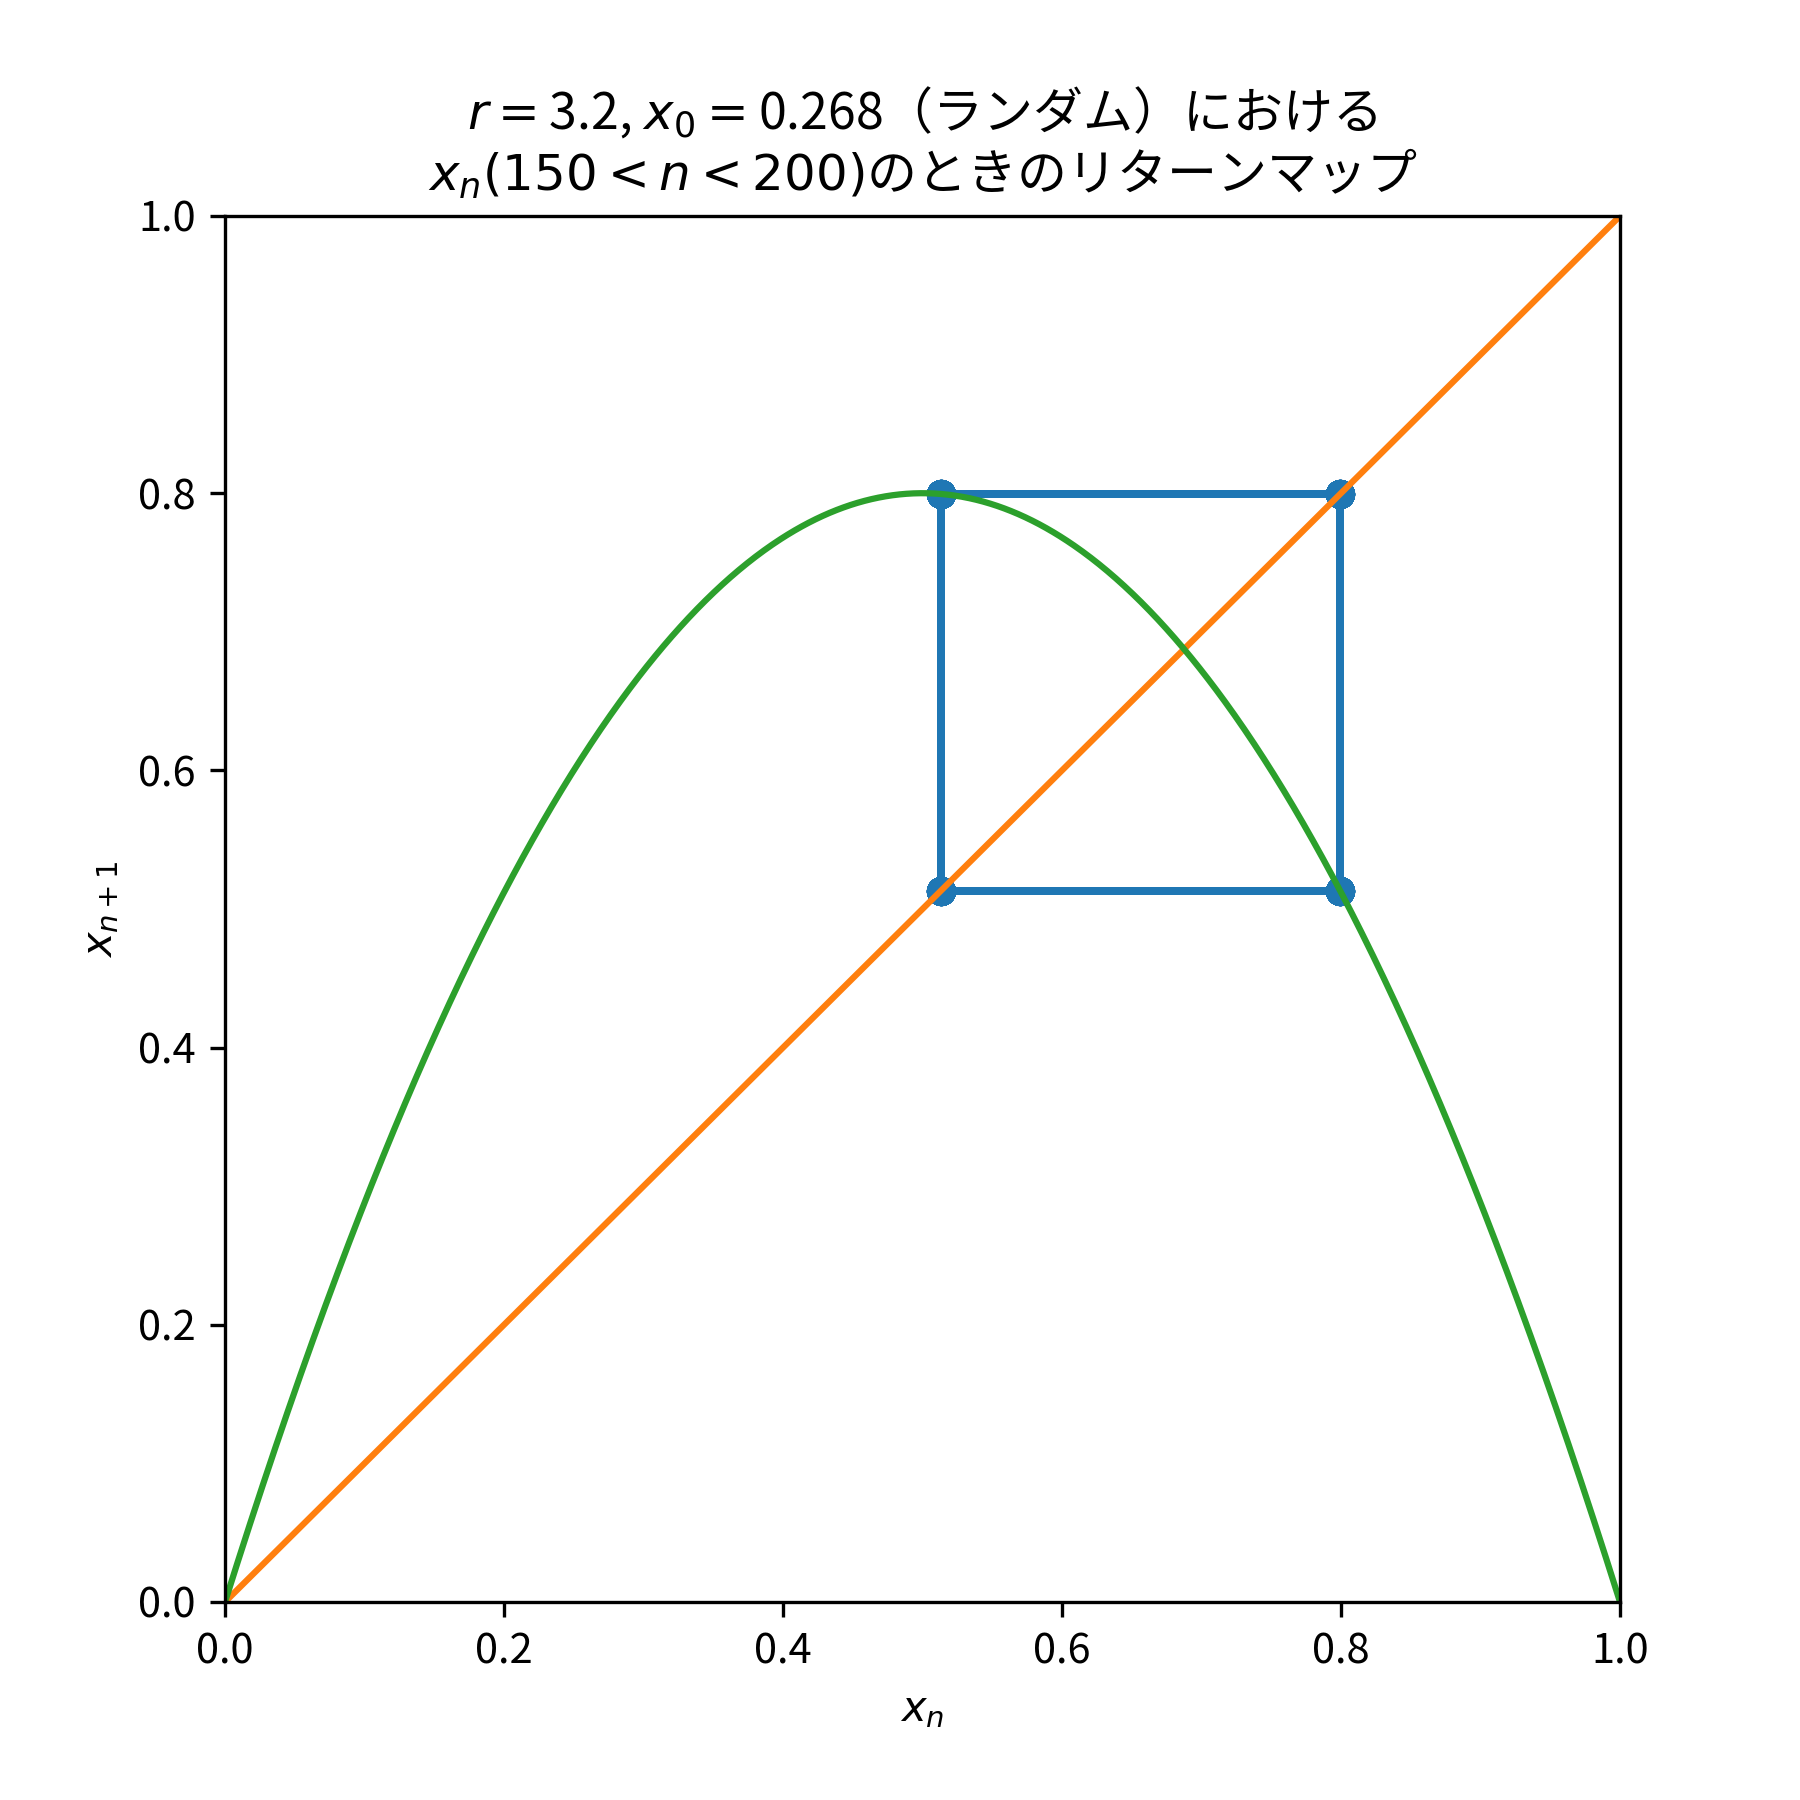
\includegraphics[keepaspectratio, scale=0.3]{images/Problem3/report4_3.png}
    \end{minipage} &
    \begin{minipage}[t]{0.45\hsize}
      \centering
      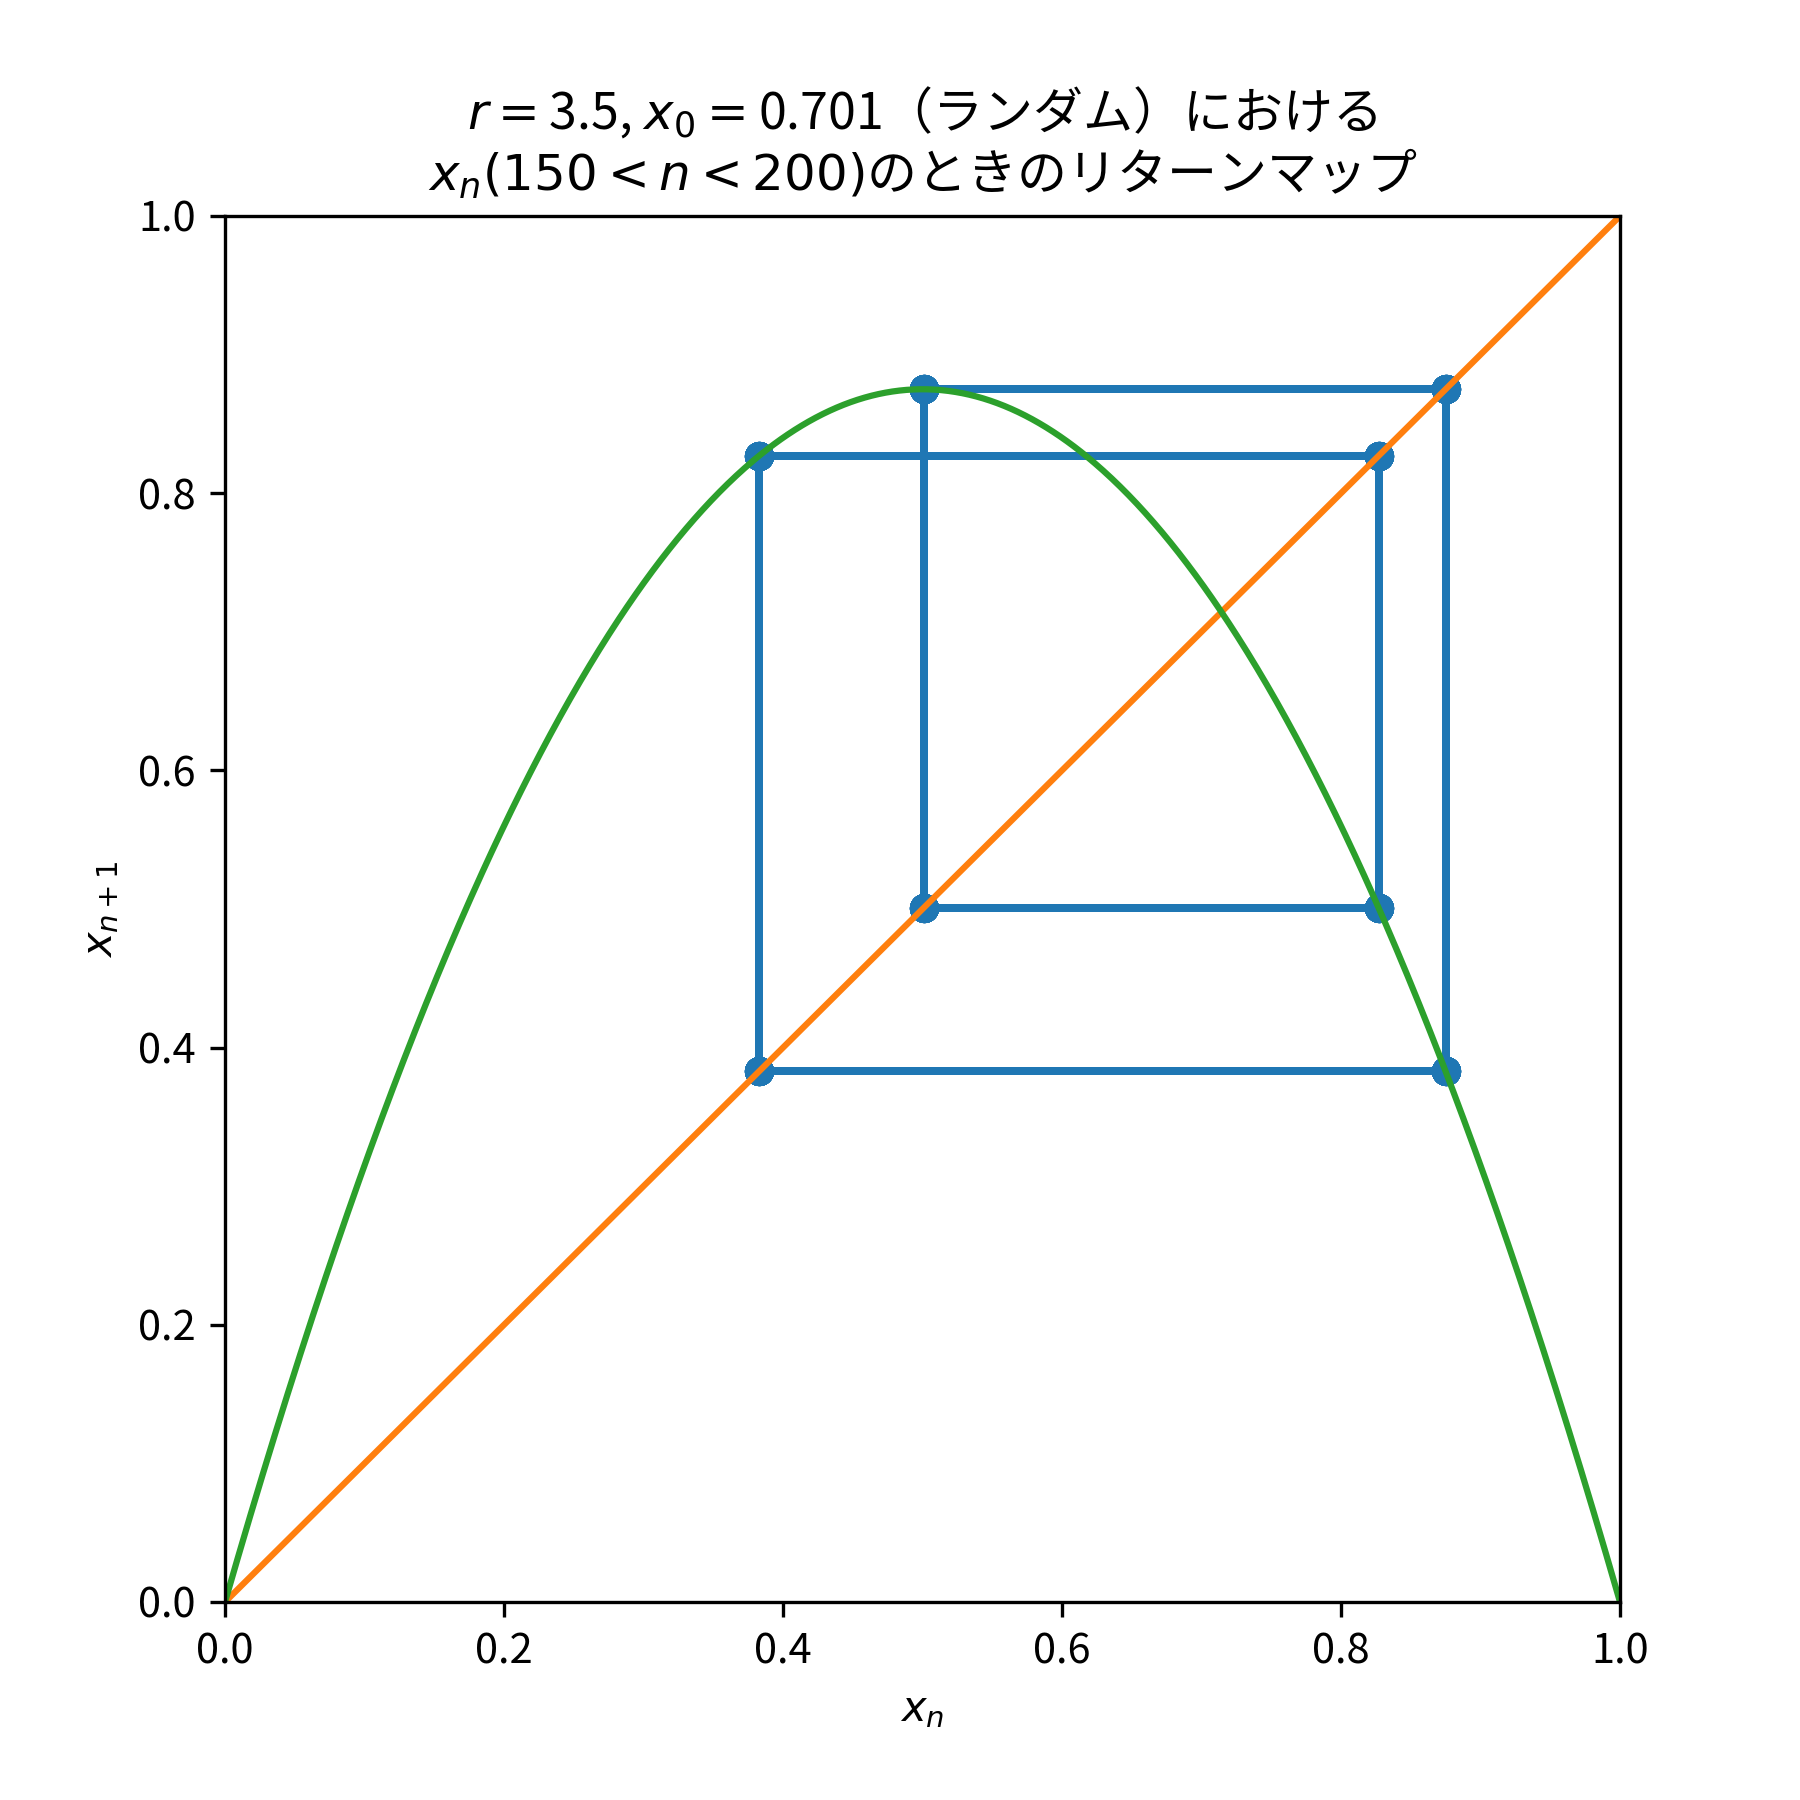
\includegraphics[keepaspectratio, scale=0.3]{images/Problem3/report4_4.png}
    \end{minipage} \\

    \begin{minipage}[t]{0.45\hsize}
      \centering
      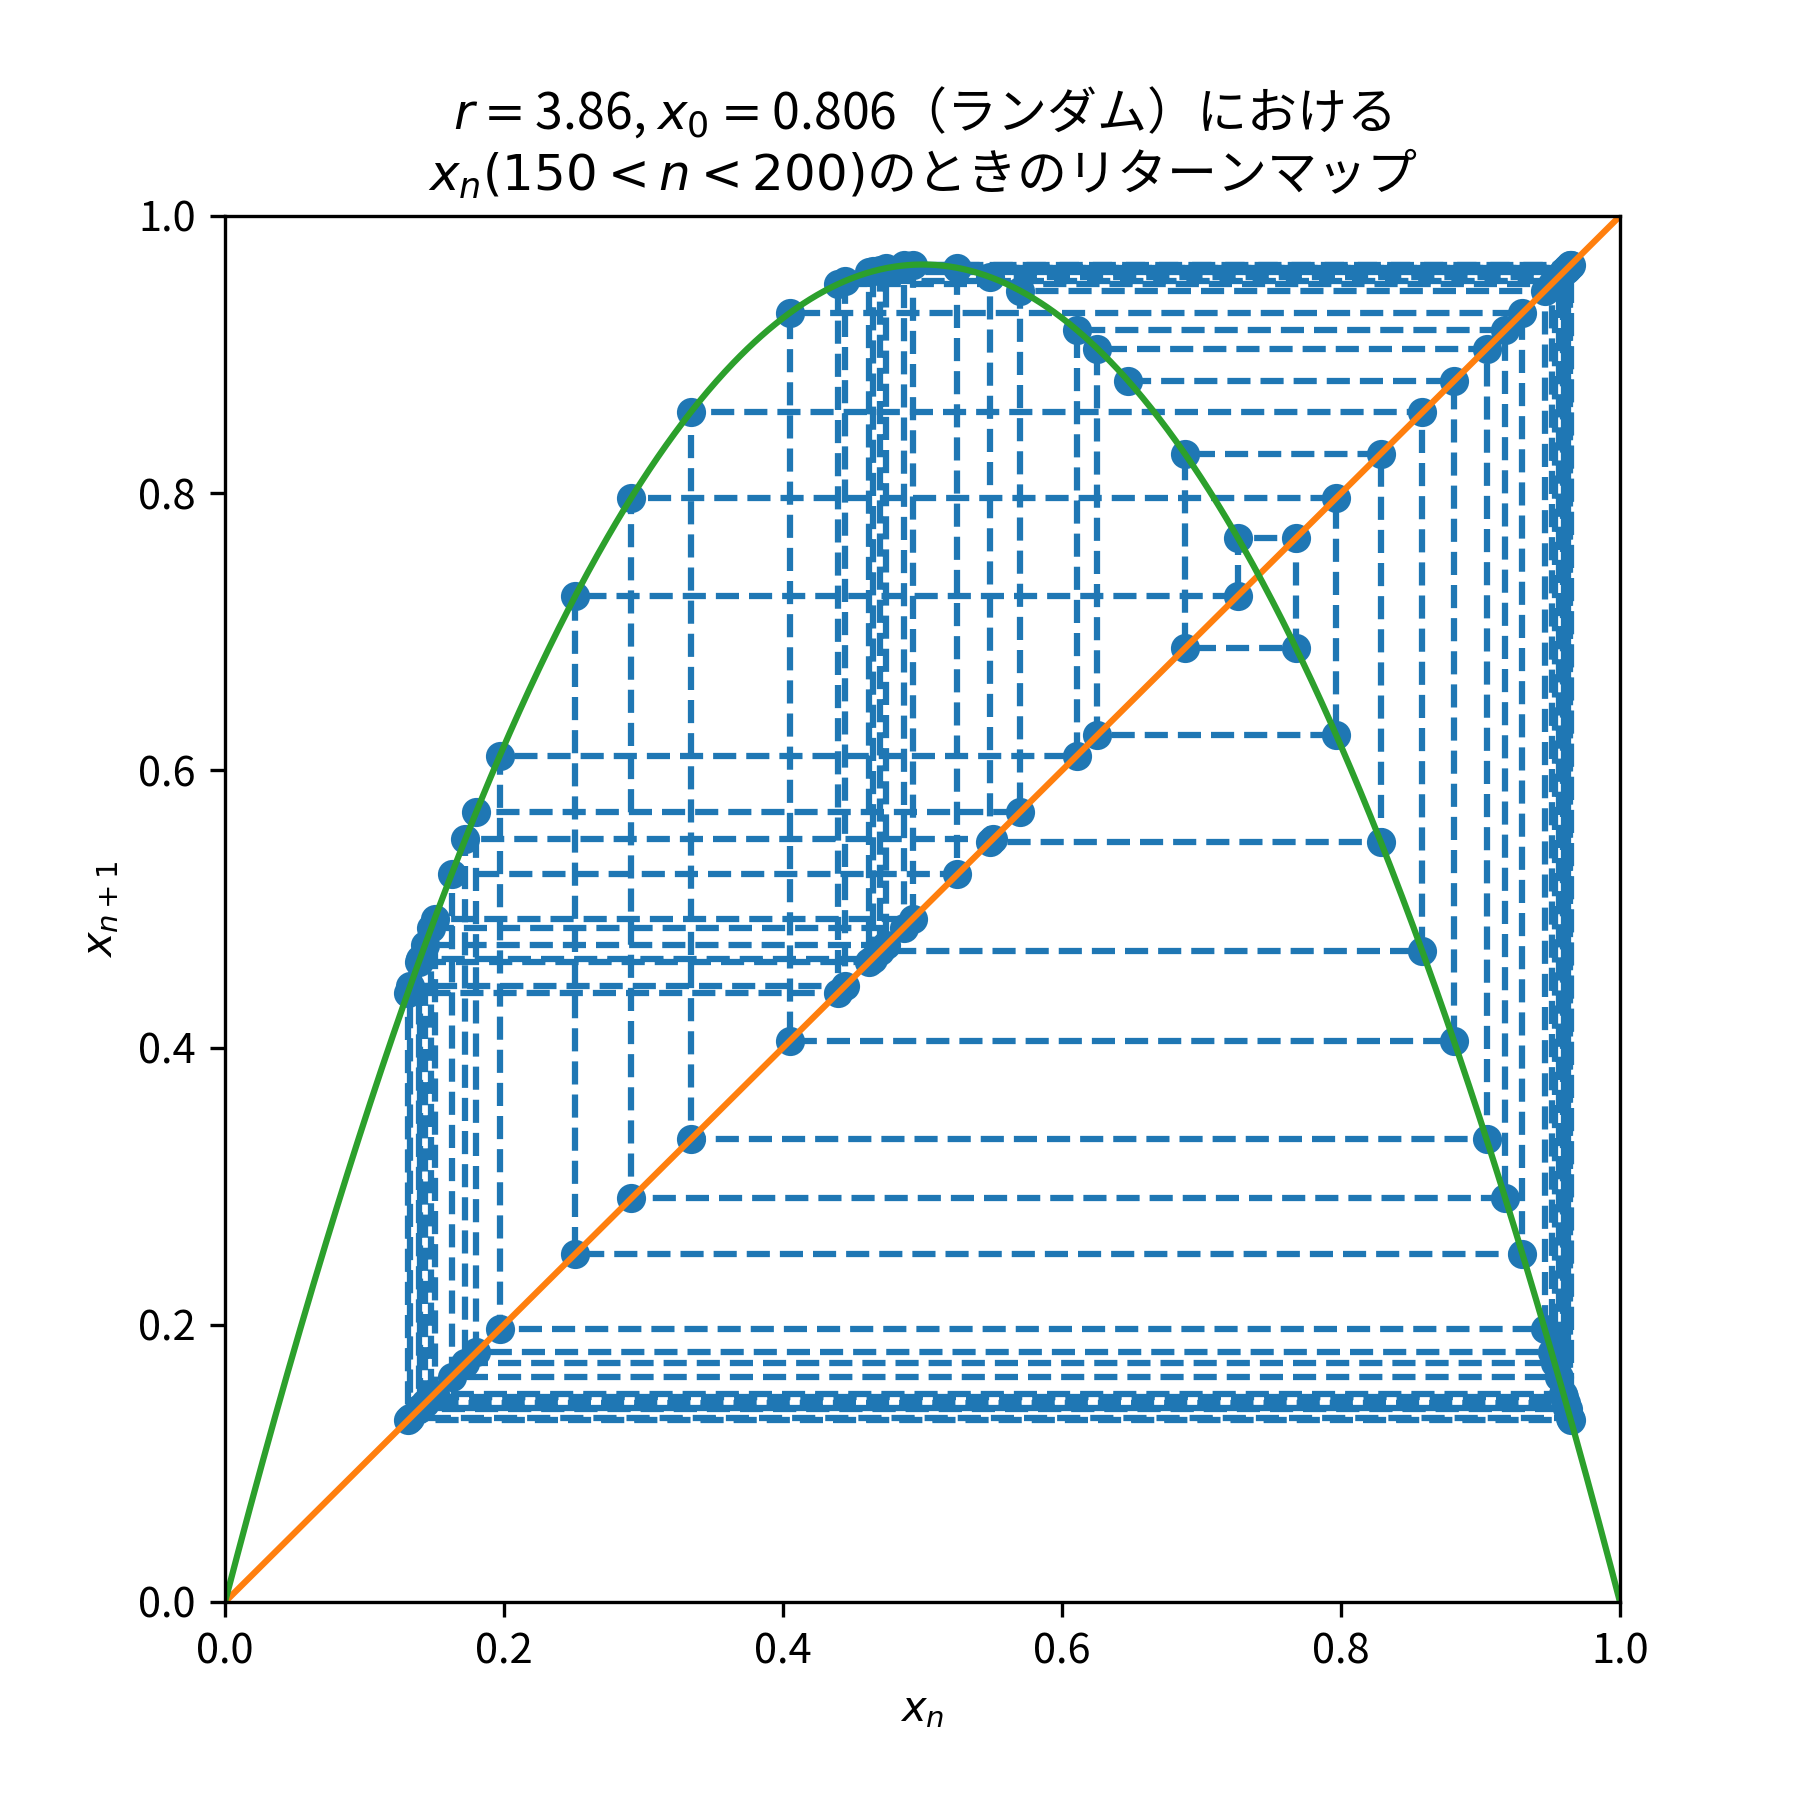
\includegraphics[keepaspectratio, scale=0.3]{images/Problem3/report4_5.png}
    \end{minipage} &
    \begin{minipage}[t]{0.45\hsize}
      \centering
      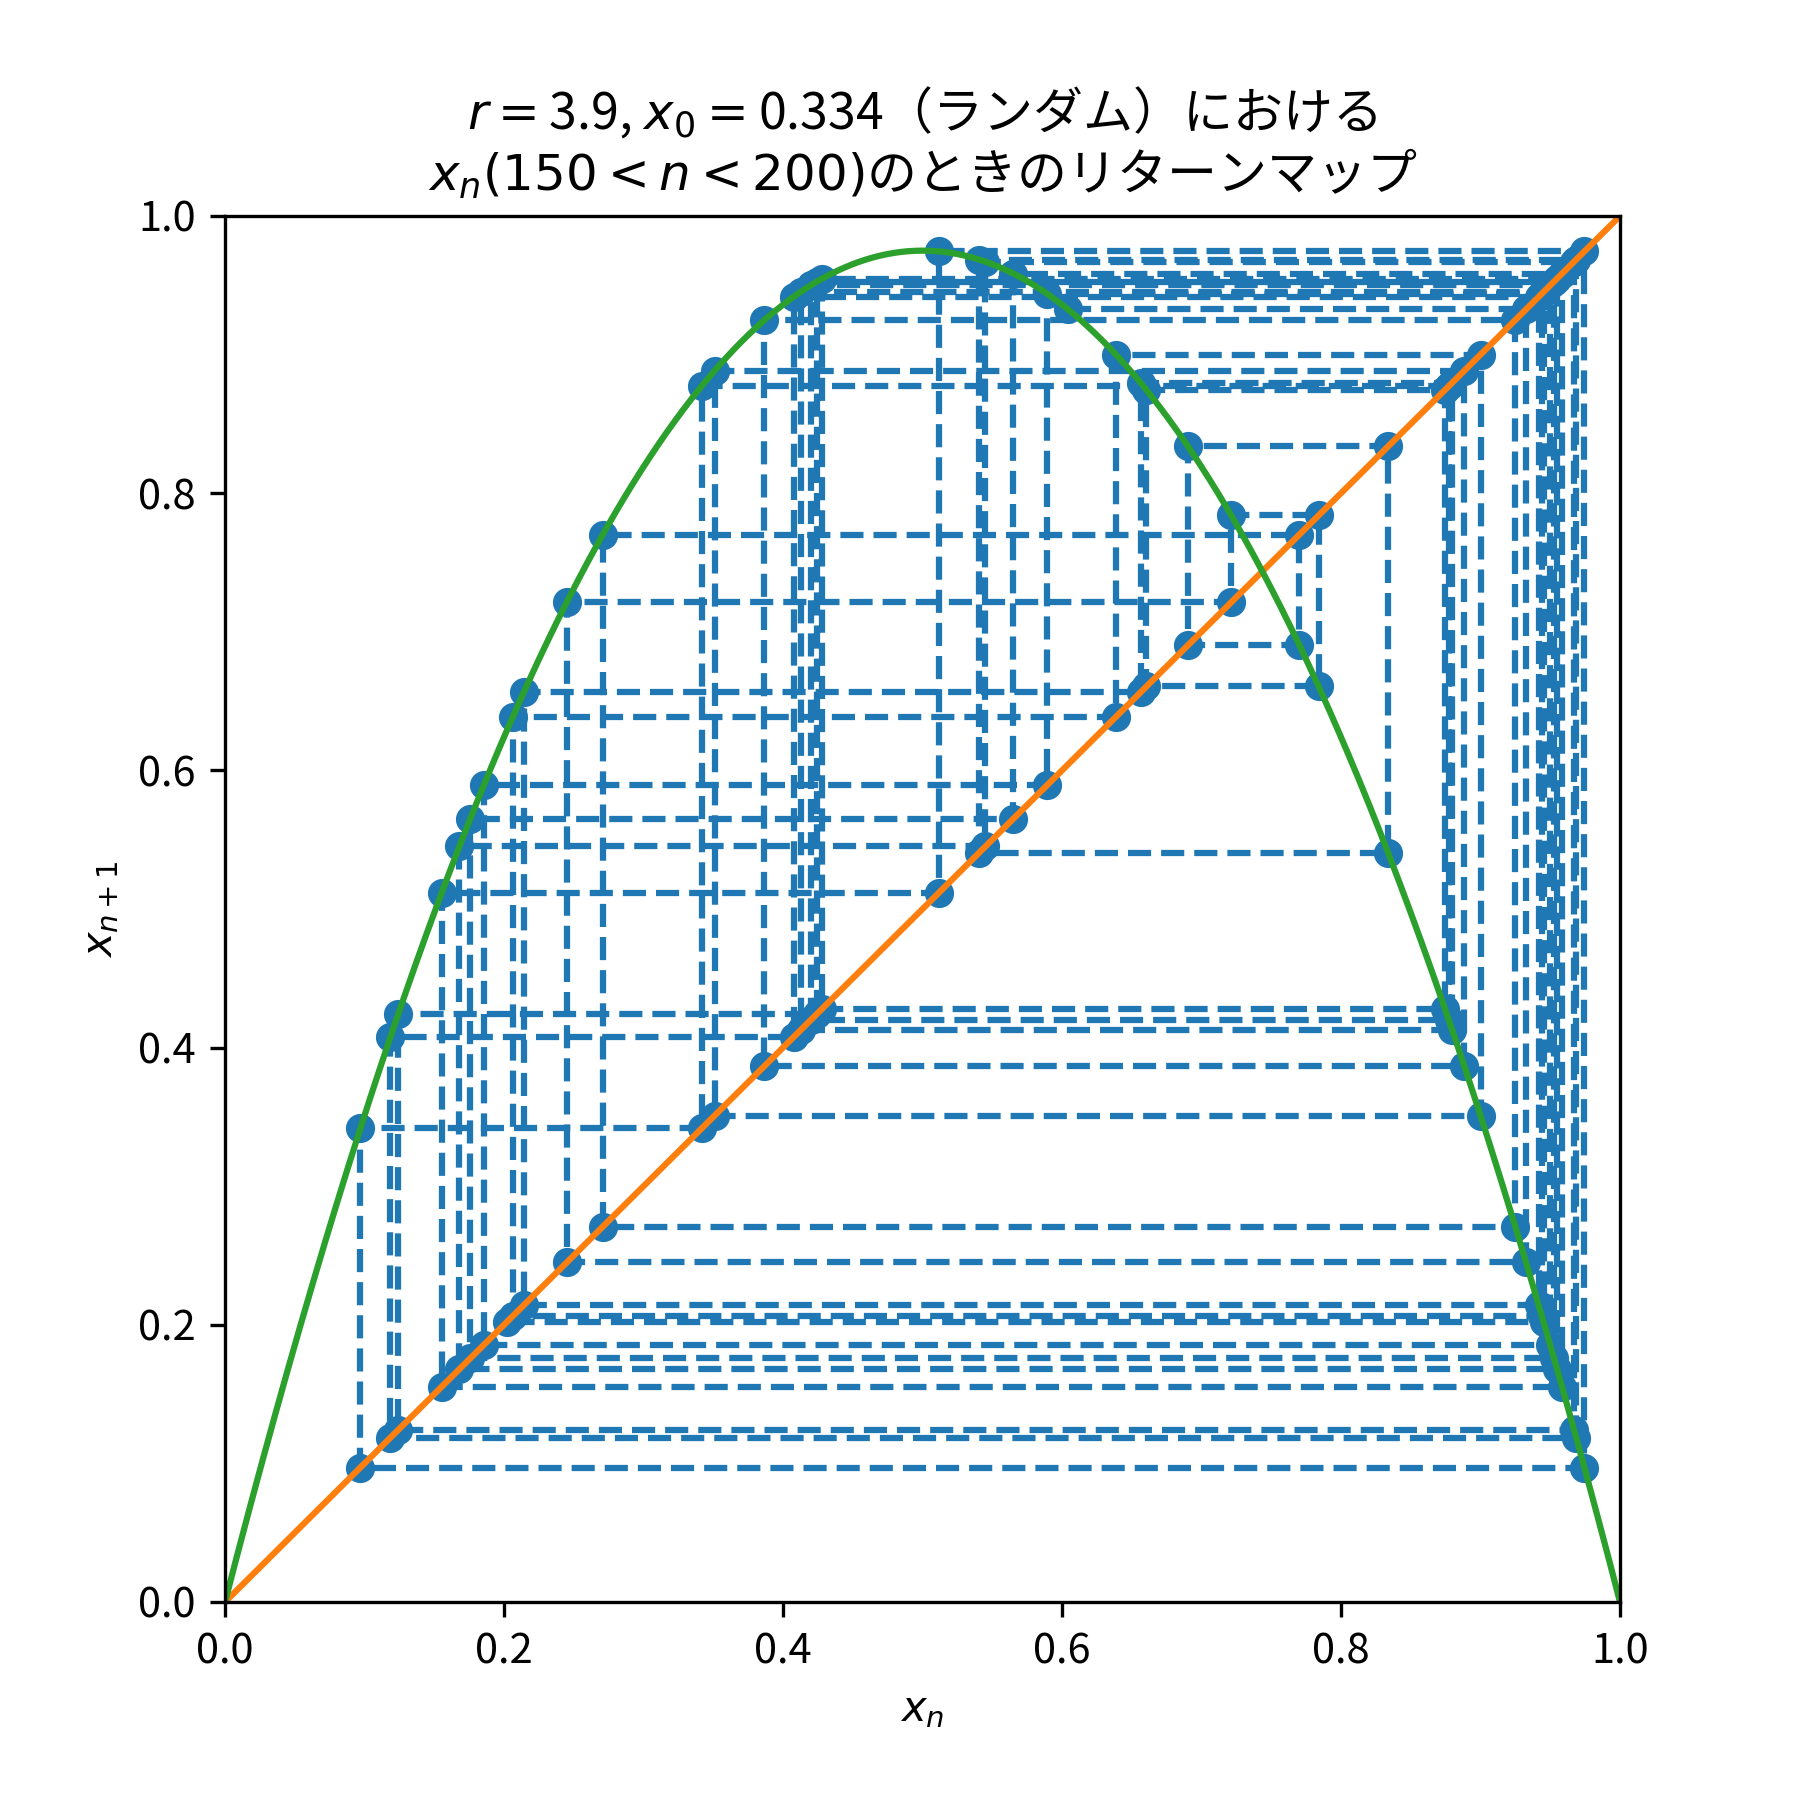
\includegraphics[keepaspectratio, scale=0.3]{images/Problem3/report4_6.png}
    \end{minipage}
  \end{tabular}
\end{figure}
\\
結果:\\
この画像から $r = 1.50, r = 2.60, r = 3.20, r = 3.50$ のときはある値を反復するようなリターンマップになっている。また、$r = 3.86, r = 3.90$ のときはある値に定まることなく個体数が変化していることが読み取れた。\\
考察:\\
レポートに添付しているランダムの値の他にもいくつかの値で実行してみたがやはり $r = 1.50, r = 2.60, r = 3.20, r = 3.50$ のときはある値を反復し $r = 3.86, r = 3.90$ のときは値が定まることなく変化していた。\\
これらの結果から $r = 3.86, r = 3.90$ のときはカオスの条件のひとつである非周期性が満たされていると考察することができる。


\subsection{課題2}
$r$ が $1~4$ のときのロジスティク写像の分岐図を描け。また、分岐図の中で3周期の窓が現れている $r$ の範囲を抽出して、グラフを描け。このとき、両グラフとも $r$ は各自適切な刻み幅を設定し、各 $r$ について初期値$x_0$をランダムに与えること。プログラムのソースコードは、 $r$ が $1~4$ のときの分岐図を出力するものと3周期の窓を出力するものとの2つを記載すること。\\
画像:\\
\begin{figure}[htbp]
  \centering
  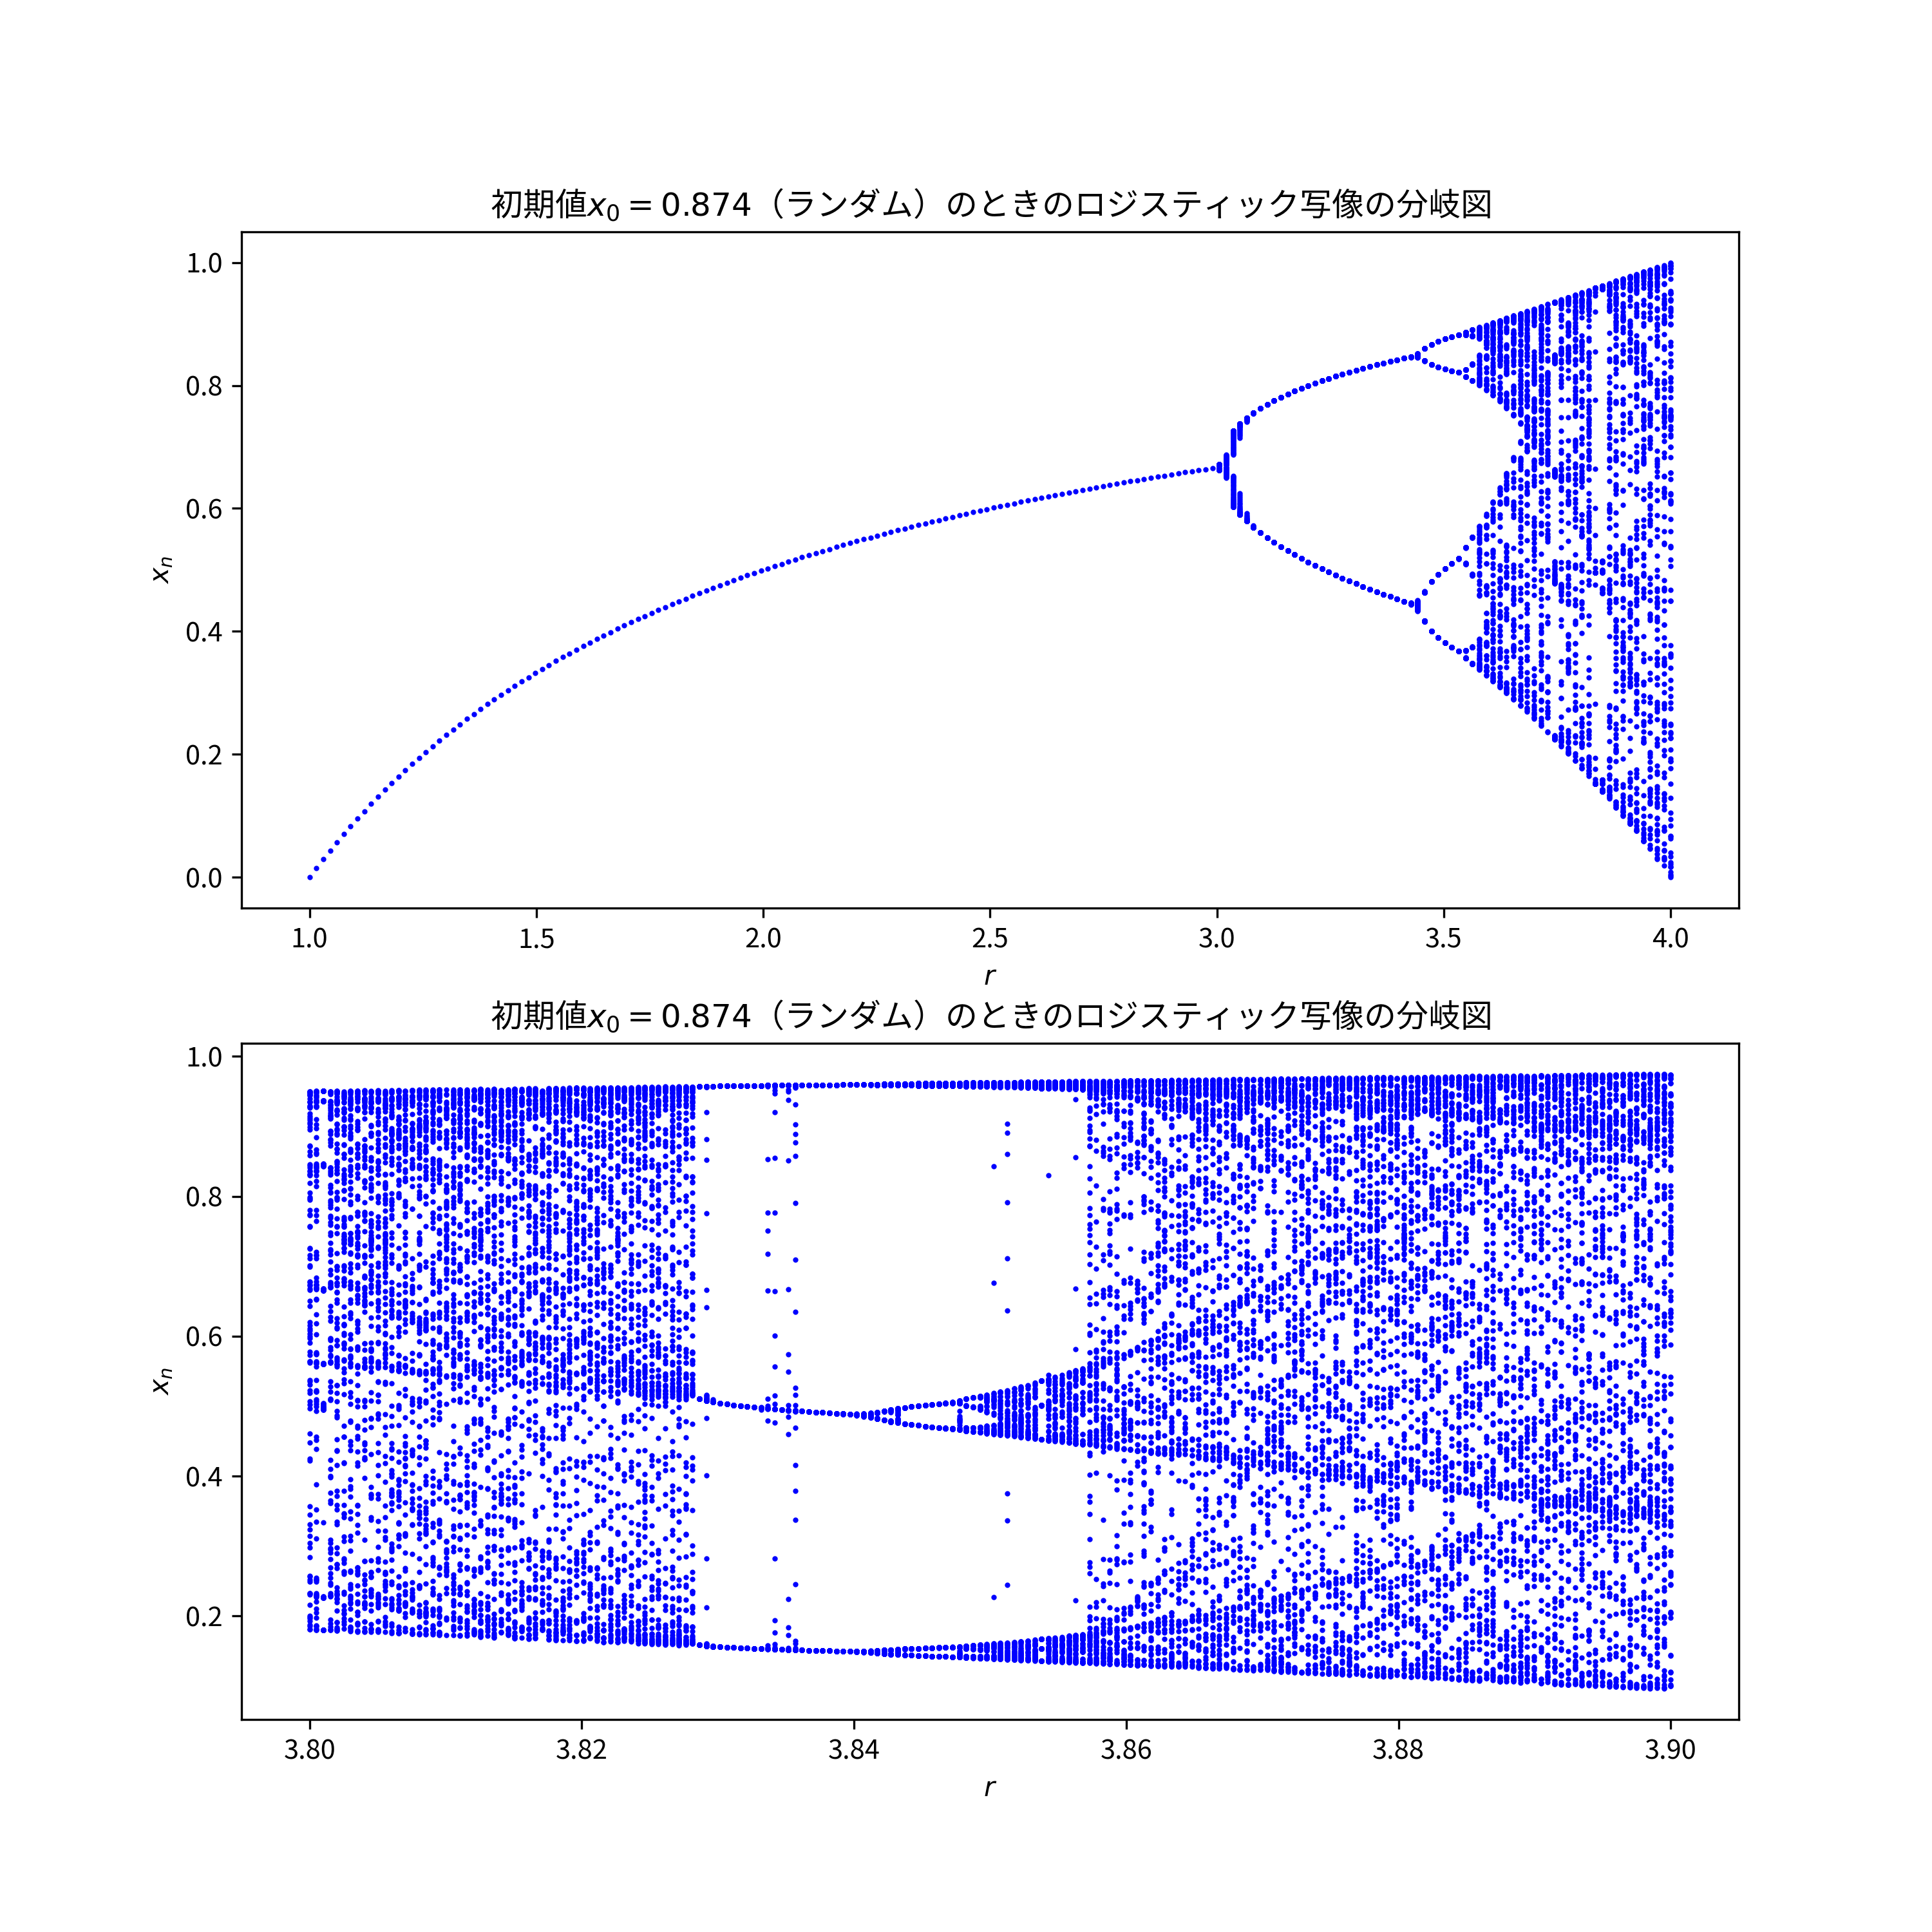
\includegraphics[keepaspectratio, scale=0.5]{images/Problem3/ctest4.png}
\end{figure}
\\
結果:\\
$r$ の刻み幅については、ロジスティック写像の分岐図では $1〜4$ を $0.02$ 刻みで値を計算しプロットした。また、3周期の窓については $3.8〜3.9$ を $0.0005$ 刻みで値を計算しプロットした。\\
この画像から $r < 3.0$ のときは1周期解のみだったが、その後 $r$ を増加していくと2周期解、4周期解、カオスのように分岐していくことが読み取れた。また、3周期の窓を見るとロジスティック写像の分岐の中で、カオスの様子を見せていた後に3周期解を持ち、またカオスの様子を見せていくことが読み取れた。\\\\
考察:\\
これらの結果から初期値 $x_0$ ではなく $r$ の値がカオスの条件と関係していると考察することができる。

\subsection{課題3}
課題1と課題2は、各 $r$ ごとに初期値 $x_0$ をランダムに与えているにもかかわらず、 $r$ が $1~3.5$ くらいまでは何度プログラムを実行しても同じようなグラフを描くことができる。一方、 $r$ が $3.5$ よりも大きくなっていくと、プログラムを実行するたびにグラフを一見するだけではわからないような違いが生じる。この理由を前回の課題と初期値鋭敏性という言葉を用いて説明せよ。\\\\
 前回の課題であるレポート課題2の課題1を見ると、$r = 3.86, r = 3.90$ のときに初期値鋭敏性があると考察した。この初期値鋭敏性によって $r = 3.5$ よりも大きくなるとランダムの初期値によってグラフが多少変化する。また、 レポート課題3の課題1では $r = 1.50, r = 2.60, r = 3.20, r = 3.50$ は初期値に関わらずある値をとっていくことが読み取れているため、$r = 3.5$ 以前では同じようなグラフになるということができる。
\subsection{ソースコード}
\begin{lstlisting}[caption=week3.py]
  from matplotlib import pyplot as plt
  import matplotlib
  import numpy as np
  import random

  # 日本語フォント用(Linux)
  matplotlib.rc('font', family='Noto Sans CJK JP')
  '''
  # 日本語フォント用(Windows)
  matplotlib.rc('font', family='MS Gothic')
  '''

  class Ctest4():
      def __init__(self) -> None:
          self.r = np.linspace(1, 4, 200, dtype=object)
          self.r2 = np.linspace(3.8, 3.9, 200, dtype=object)
          fig = plt.figure(figsize=(10, 10))
          self.ax1 = fig.add_subplot(2, 1, 1)
          self.ax2 = fig.add_subplot(2, 1, 2)

          # self.x = 0.1    # 初期値を0.1と仮定
          self.x = random.uniform(0, 1)
          # 固定点
          self.u1 = list(map(lambda x: 0, self.r))
          self.u2 = list(map(lambda x: 1 - 1 / x, self.r))
          self.u3 = list(map(lambda x: 0, self.r2))
          self.u4 = list(map(lambda x: 1 - 1 / x, self.r2))

          # 乗数
          self.lambda1 = self.r
          self.lambda2 = list(map(lambda x: 2 - x, self.r))
          self.lambda3 = self.r2
          self.lambda4 = list(map(lambda x: 2 - x, self.r2))
          
          self.filepath = "複雑系科学演習/Week4/images/"

      def proprocessing(self, r: float) -> list:
          '''グラフに入れるための前処理'''
          x_array = []
          r_array = []
          num = self.x
          for i in range(150):
              num = r * num * (1 - num)
              if i < 40:
                  continue
              x_array.append(num)
              r_array.append(r)
          return x_array, r_array

      def code_problem1(self):
          self.ax1.set_title('初期値$x_0 = {}$(ランダム)のときのロジスティック写像の分岐図'.format(round(self.x, 3)))
          self.ax1.set_xlabel('$r$')
          self.ax1.set_ylabel('$x_n$')
          for i in range(len(self.r)):
              if -1 <= self.lambda1[i] <= 1:
                  self.ax1.scatter(self.r[i], self.u1[i], color='b', s=1)
              elif -1 <= self.lambda2[i] <= 1:
                  self.ax1.scatter(self.r[i], self.u2[i], color='b', s=1)
              else:
                  result = self.proprocessing(self.r[i])
                  self.ax1.scatter(result[1], result[0],  color='b', s=1)

      def code_problem2(self):
          self.ax2.set_title('初期値$x_0 = {}$(ランダム)のときのロジスティック写像の分岐図'.format(round(self.x, 3)))
          self.ax2.set_xlabel('$r$')
          self.ax2.set_ylabel('$x_n$')
          for i in range(len(self.r2)):
              if -1 <= self.lambda3[i] <= 1:
                  self.ax2.scatter(self.r2[i], self.u3[i], color='b', s=1)
              elif -1 <= self.lambda4[i] <= 1:
                  self.ax2.scatter(self.r2[i], self.u4[i], color='b', s=1)
              else:
                  result = self.proprocessing(self.r2[i])
                  self.ax2.scatter(result[1], result[0],  color='b', s=1)

      def save_fig(self):
          plt.savefig(self.filepath + 'ctest4', dpi=300)
          plt.show()

      def do_plot(self):
          self.code_problem1()
          self.code_problem2()
          self.save_fig()

  class Report_3():
      def __init__(self, r: float, s: str) -> None:
          self.r = r
          self.s = s
          self.x = random.uniform(0, 1)
          self.xn = np.linspace(0, 1, 1000)
          self.filepath = "複雑系科学演習/Week4/images/"

      def logistic(self, x: float, cnt: int) -> list:
          num = x
          num_array = [x]
          for i in range(cnt):
              num = self.r * num * (1 - num)
              num_array.append(num)
          return num_array

      def pre_processing(self, cnt: int) -> float:
          '''初期変動の影響をなくすための前処理'''
          num = self.x
          for i in range(cnt):
              num = self.r * num * (1 - num)
          return num

      def plot_return_map(self):
          '''初期変動が影響しないリターンマップの描画'''
          plt.figure(figsize=(6, 6))
          # 処理
          x = self.pre_processing(150)
          n = self.logistic(x, 50)
          xn_array = []
          for i in self.xn:
              xn_array.append(self.r * (1 - i) * i)
          # クモの巣図用の配列
          spiper_plot_x = []
          spiper_plot_y = []
          for i in range(1, len(n)):
              spiper_plot_x.append(n[i - 1])
              spiper_plot_x.append(n[i])
              spiper_plot_y.append(n[i])
              spiper_plot_y.append(n[i])
          
          plt.plot(spiper_plot_x, spiper_plot_y, marker='o', linestyle='dashed')
          plt.plot(self.xn, self.xn)
          plt.plot(self.xn, xn_array)
          plt.title("$r = $" + str(self.r) + ", $x_0 = $" + str(round(self.x, 3)) + '(ランダム)における\n' +\
              '$x_n (150 < n < 200)$のときのリターンマップ')
          plt.xlim(0, 1)
          plt.ylim(0, 1)
          plt.xlabel("$x_n$")
          plt.ylabel("$x_{n+1}$")
          plt.savefig(self.filepath + self.s, dpi=300)


  r = [1.50, 2.60, 3.20, 3.50, 3.86, 3.90]

  demo = Ctest4()
  # demo.do_plot()
  for i in range(len(r)):
      demo = Report_3(r[i], "report4_{}".format(i + 1))
      demo.plot_return_map()
\end{lstlisting}